
\documentclass[aps,prl,reprint]{revtex4-2}

\usepackage{graphicx}
\usepackage{hyperref}
\hypersetup{colorlinks=true, citecolor=blue, urlcolor=blue, linkcolor=blue}


\begin{document}

% Use the \preprint command to place your local institutional report
% number in the upper righthand corner of the title page in preprint mode.
% Multiple \preprint commands are allowed.
% Use the 'preprintnumbers' class option to override journal defaults
% to display numbers if necessary
%\preprint{}

%Title of paper
\title{My lab report}

% repeat the \author .. \affiliation  etc. as needed
% \email, \thanks, \homepage, \altaffiliation all apply to the current
% author. Explanatory text should go in the []'s, actual e-mail
% address or url should go in the {}'s for \email and \homepage.
% Please use the appropriate macro foreach each type of information

% \affiliation command applies to all authors since the last
% \affiliation command. The \affiliation command should follow the
% other information
% \affiliation can be followed by \email, \homepage, \thanks as well.
\author{Trevor Smith}
\email[]{smith.tr@northeastern.edu}
%\homepage[]{Your web page}
%\thanks{}
%\altaffiliation{}
\affiliation{Northeastern University}


\date{\today}

\begin{abstract}
The abstract contains a brief summary of one short paragraph with only 4 to 8 sentences. Basically, it gives an overview of: (1) specifically what you did; (2) what you found (including final values with uncertainties); and (3) comparison to expected values. This is your first selling point. If you don’t catch the reader’s attention here, they may not be motivated to read the rest of the report. Keep it simple.
\end{abstract}


\maketitle

% body of paper here - Use proper section commands
% References should be done using the \cite, \ref, and \label commands
\section{Introduction}

This course provides writing credit (NU Core Writing Intensive in the Major), so everyone should write their own lab report. You can share the data with your lab partner, but each student should do their own analysis and make their own plots and tables.

Writing lab reports for your physics classes gives you valuable experience, as you will eventually write reports for your employers, submit grants to funding agencies, and submit papers for scientific journals. Here are some very important, but simple ingredients to keep in mind when writing a report.

Try to separate in your mind the most important item from the less-important details. Readers don’t want to spend the time figuring out what is important. For example, if you measure the speed of light in glass (v), the important result is the refractive index (n = v/c), not the speed.

Keep an eye on the organization. Keep parts together that need to be together. For example, if you give a long list of procedures, then a long list of results, the reader will have to go back and forth between the sections. Use section and subsection headings where necessary.

The Introduction should contain 1 or 2 paragraphs. Briefly state the physics underlying the experiment (what is being tested and why). 

\section{Apparatus}

List equipment components (manufacturer, model numbers and brief specifications). 

The apparatus consisted of the following.
\begin{itemize}
\item Oscilloscope, Tektronix TDS210 
\item Multimeter, GMW1405
\item Electromagnet, GMW3633
\item Lens, 25 mm focal length
\end{itemize}

Include diagrams or sketches of important apparatus and number them (label items and describe in the text or caption). You can put the figure and the caption in a ``test box.''

\section{Procedures and Results}

Since there are several parts of each experiment, it is better to discuss the procedures, results and conclusions for each part before going on to the next part.  For each part of the experiment include the following. 

\begin{itemize}
\item Briefly describe the experimental procedures (in your own words, but don’t overdo it)
\item Discuss calibrations, etc., if required
\item Include necessary equations and put them on their own line (number them, e.g. “Eq. (3)”)
\item Include plots showing relevant results (label each figure, e.g. “Fig. 3”, with caption).
\item Describe what you found (describe what the plot illustrates)
\end{itemize}

\begin{figure}
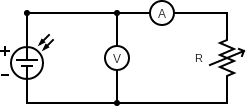
\includegraphics[width=0.4\textwidth]{circuit.png}
\caption{\label{circuitdiagram}Electrical circuit for measuring photovoltaic (PV) output voltage and current through a variable resistor (R).}
\end{figure}


\subsection{Figures}

\begin{itemize}
\item Figures are usually no larger than 3-4” wide
\item When you have a plot, put the data table into an Appendix at the end
\item Axis titles and numbers must be large enough to be easily read
\item Plot only the “region of interest” (ROI) – think about what you are trying to show (However, in a few cases you may want to show where zero is on the axis, as for the Ruby transmission)
\item Connect data points by a line, as a guide for the eye
\item Include curve fits to the data; plot the theory whenever possible (theory is usually a curve and the data are points)
\end{itemize}

\begin{figure}
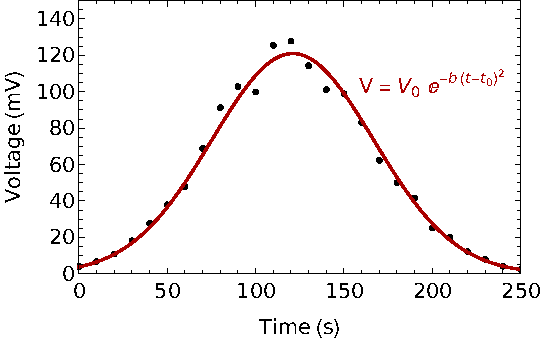
\includegraphics[width=0.46\textwidth]{plot.pdf}
\caption{\label{plot}Peak voltage as a function of time for photon counting experiment. The curve is a fit of the data points to a Gaussian function.}
\end{figure}

\subsection{Computations}

\begin{itemize}
\item List all necessary equations (number them, “Eq. (4)”), define all variables and constants 
\item List measured values that are input into equations, such as distance, current, voltage, etc.
\item If you have a plot with more than 4-5 points, you do not need to include a table of data in the report (but you can put tables in an Appendix at the end)
\item Compute uncertainties for all important final results
\end{itemize}

Example: The reflectivity ($R$) of an air-medium interface is given by
\begin{equation} 
R = \frac{ (n-1)^2 } { (n+1)^2 },
\label{reflectivity}
\end{equation}
%
where $n$ is index of refraction of the medium \cite{wiki-spectroscopy}. For crown glass $n = 1.5$ . By using eqn. (\ref{reflectivity}),  the reflectivity for one surface is found to be $R = 4\%$.

\section{Summary}

Here is where you wrap up the experiment. This is usually a somewhat expanded version of the abstract, but has several things added. Include the following. 

\begin{itemize}
\item Discuss (briefly) the interpretation of each result
\item Make a table of all important results (values) with uncertainties and expected/accepted values
\item List references for accepted values, etc.
\item Compare your results to accepted values
\item Discuss the major contributions to the uncertainties
\end{itemize}

\begin{widetext}
\begin{center}
\begin{table}[h]
\renewcommand{\arraystretch}{1.35}
\setlength{\tabcolsep}{10pt}
\caption{\label{}Measured and accepted values of the speed of light and refractive index of various materials.}
\begin{tabular}{|c|c|c|c|c|c|}
%\hline
\toprule
Material & $v$ (m/s) & $n$ & Accepted $n$ value & Refs. & Deviation \\
\colrule
Air & $(2.92 \pm 0.06) \times 10^8$  & $0.97 \pm 0.02$ & $n=1.00$ & \cite{Hollingsworth} & $-2 \sigma$ \\
\colrule
Water & $(2.36 \pm 0.08) \times 10^8$  & $1.27 \pm 0.04$ & $n=1.33$ & \cite{Benford} & $-2\sigma$  \\
\colrule
Glass & $(2.92 \pm 0.06) \times 10^8$  & $1.55  \pm 0.10$ & $n = 1.50$ & \cite{Hollingsworth} & $\phantom{-}1 \sigma$ \\
%\hline
\botrule
\end{tabular}
\end{table}
\end{center}
\end{widetext}





\begin{thebibliography}{9}
%
\bibitem{wiki-spectroscopy} 
Wikipedia, Spectroscopy: \\
\href{http://en.wikipedia.org/wiki/Spectroscopy}{http://en.wikipedia.org/wiki/Spectroscopy}
%
\bibitem{Hollingsworth} 
G. Hollingsworth, \textit{“Optical Physics”}, (Wiley and Sons, New York, 2015).
%
\bibitem{Benford} 
M.J. Benford, R.W. Smith, and L.L. Liu,  
\textit{“Optical measurement of water,”}
Phys. Rev. 14, 516 (1835)
%
\end{thebibliography}


\end{document}
%
% ****** End of file apstemplate.tex ******

